\documentclass[final]{beamer}
\usepackage{hyperref,xspace,graphicx,microtype,minted,
multicol,mflogo,enumerate,mathtools,hologo,xcolor,tcolorbox,ccicons,calc}
\usepackage[brazil]{babel}
\usepackage{fontspec}

\usetheme[subsectionpage=progressbar,numbering=none]{metropolis}
\beamertemplatenavigationsymbolsempty

% Macros
\newcommand{\filename}[1]{\texttt{#1}}
%
\newcommand{\code}[1]{\texttt{#1}}
%
\newcommand{\email}[1]{\href{mailto:#1} {\texttt{\textless#1\textgreater}}
}
%
\newmintinline[latexcode]{latex}{}
%
\newcommand{\todo}[1]{\colorbox{yellow}{#1}}

\title{Introdução ao \LaTeX}
\author{Rafael Beraldo \qquad \email{rberaldo@cabaladada.org}}
\date{20 e 20 de setembro de 2018}

\begin{document}
\maketitle

% Conteúdo
\begin{frame}
  \frametitle{Conteúdo}
  \setbeamertemplate{section in toc}[sections numbered]
  \begin{multicols}{2}
    \tableofcontents
  \end{multicols}
\end{frame}

% História %%%%%%%%%%%%%
\section{História}

\begin{frame}[plain]
  \begin{figure}[h]
    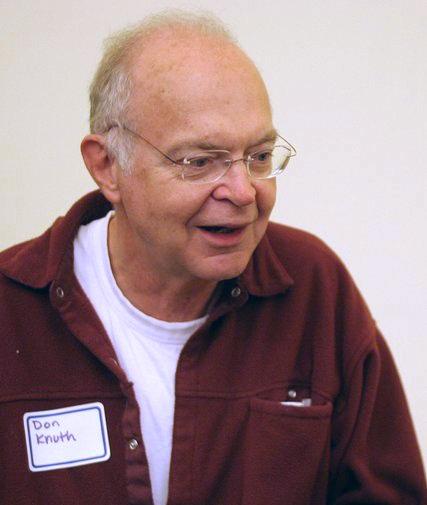
\includegraphics[scale=.5]{imagens/knuth}
    \caption{Donald Knuth em 2005}
  \end{figure}
\end{frame}

\begin{frame}[plain]
  \hspace*{-11.5mm}
  \begin{centering}
    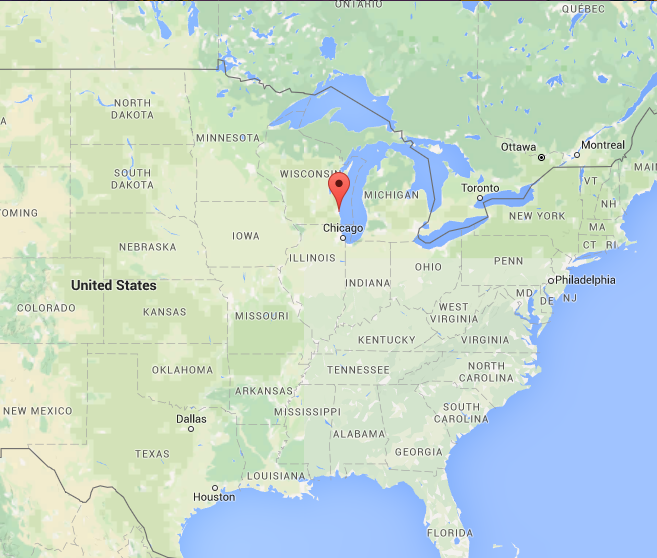
\includegraphics[width=\pagewidth]{imagens/milwaukee}
  \end{centering}
\end{frame}

\begin{frame}
  \frametitle{História do LaTeX}
  \LARGE
  \only<1>{O pai de Knuth\\ tinha uma editora}
  \only<2>{1977: segunda edição do segundo volume de \emph{The Art of Computer
  Programming}}
  \only<3>{\textsc{ascii} não foi projetado\\ com livros em mente}
  \only<4>{\TeX: tau epsilon chi}
\end{frame}

\begin{frame}
  \large
  \begin{quote}
    The purpose of this pronunciation exercise is to remind you that \TeX\ is
    primarily concerned with high-quality technical manuscripts: Its emphasis
    is on art and technology, as in the underlying Greek word. If you merely
    want to produce a passably good document—something acceptable and basically
    readable but not really beautiful—a simpler system will usually suffice.
    With \TeX\ the goal is to produce the finest quality; this requires more
    attention to detail, but you will not find it much harder to go the extra
    distance, and you’ll be able to take special pride in the finished
    product.\hfill (Donald Knuth, \emph{\TeX book})
  \end{quote}
\end{frame}

\begin{frame}
  \frametitle{História do LaTeX}
  \LARGE
  \LaTeX: 1985
\end{frame}

\begin{frame}[plain]
  \begin{figure}[h]
    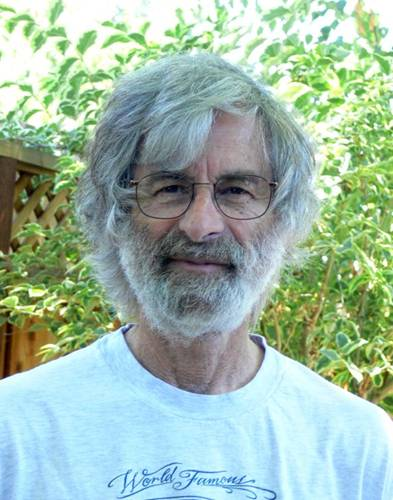
\includegraphics[scale=.5]{imagens/lamport}
    \caption{Leslie Lamport}
  \end{figure}
\end{frame}

% LaTeX: uma linguagem de marcação %%%%%%%%%%%%%%
\section[\LaTeX: uma linguagem de marcação]{Linguagem de marcação}

% O LaTeX é uma linguagem de marcação de texto, ou markup
\begin{frame}
  \frametitle{\LaTeX: uma linguagem de marcação}
  \LARGE
  \only<1>{\LaTeX{} é uma linguagem de \emph{markup}}
  \only<2>{Você \emph{declara} o documento}
  \only<3>{O programa segue as instruções}
  \only<4>{Assim como em \textsc{html},\\ o arquivo fonte é renderizado}
  \only<5>{Comandos são semânticos}
\end{frame}

% Se os comandos são semânticos, devem ser fáceis de interpretar. O que os
% comandos abaixo significam?
\begin{frame}[fragile]
  \frametitle{\LaTeX: uma linguagem de marcação}
  \begin{minted}[autogobble,fontsize=\LARGE,breaklines]{latex}
    \tableofcontents

    \section{Introdução}
  \end{minted}
\end{frame}

% Arquivos .tex não contém formatação; são texto plano.
\begin{frame}
  \frametitle{\LaTeX: uma linguagem de marcação}
  \LARGE
  \code{.tex} são arquivos de texto plano
\end{frame}

% Exemplo de artigo %%%%%%%%%%%%%%
\section{Exemplo de artigo}

% Vejamos nosso primeiro artigo em LaTeX.
\begin{frame}
  \frametitle{Exemplo de artigo}
  \Huge
  Vejamos \filename{exemplo/artigo.tex}
\end{frame}

% Comandos %%%%%%%%%%%%%%
\section{Comandos}

% Comandos simples não têm argumentos
\begin{frame}[fragile]
  \frametitle{Comandos simples}
  \begin{minted}[autogobble,fontsize=\LARGE,breaklines]{latex}
    \tableofcontents
  \end{minted}
\end{frame}

% Comandos simples e espaço em branco
\begin{frame}[fragile]
  \frametitle{Comandos simples e espaço em branco}
  \begin{minted}[autogobble,fontsize=\LARGE,breaklines]{latex}
    \tableofcontents Isso funciona
  \end{minted}
\end{frame}

\begin{frame}[fragile]
  \frametitle{Comandos simples e espaço em branco}
  \begin{minted}[autogobble,fontsize=\LARGE,breaklines]{latex}
    \tableofcontents
    Melhor agora
  \end{minted}
\end{frame}

% Comandos com argumentos
\begin{frame}[fragile]
  \frametitle{Comandos com argumento}
  \begin{minted}[autogobble,fontsize=\normalsize,breaklines]{latex}
    \section{Introdução}\label{introducao}Também funciona
  \end{minted}
\end{frame}

% Voltemos ao exemplo para demonstrar
\begin{frame}
  \frametitle{Exemplos de comandos}
  \huge
  Vejamos \filename{exemplo/artigo.tex} novamente
\end{frame}

% Espaço em branco %%%%%%%%%%%%%%
\subsection{Espaço em branco}

% Espaços em branco são condensados
\begin{frame}[fragile]
  \frametitle{Espaços em branco}
  \begin{minted}[autogobble,fontsize=\normalsize,breaklines]{latex}
    \section      {Introdução}
        \label{introducao}

        Este exemplo funciona, mas o código não é
     muito legível.  O resultado será perfeito, entretanto.
  \end{minted}
\end{frame}

% Voltemos ao exemplo para aprender mais sobre espaços em branco e como usá-lo
% de maneira a deixar seu código mais legível.
\begin{frame}
  \frametitle{Espaços em branco}
  \huge
  Vejamos \filename{exemplo/artigo.tex}
\end{frame}

% Vamos resolver nosso primeiro exercício e compilar o arquivo. Haverá um
% problema com hifenização.
\begin{frame}
  \frametitle{Espaços em branco}
  \huge
  Resolver \filename{exercicios/espaco\-branco.tex}
\end{frame}

% Símbolos especiais %%%%%%%%%%%%%%
\section{Símbolos especiais}

% Aspas
\begin{frame}[fragile]
  \frametitle{Aspas}
  \begin{minted}[autogobble,fontsize=\LARGE,breaklines]{latex}
    ``Devemos abrir aspas com dois acentos graves e fechar com duas aspas
    simples.''
  \end{minted}
\end{frame}

% Traços
\begin{frame}[fragile]
  \frametitle{Hífen, travessão e meia-risca}
  \begin{minted}[autogobble,fontsize=\LARGE,breaklines]{latex}
    Leve um guarda-chuva --- ouvi na rádio que pode chover entre 10h--13h.
  \end{minted}
\end{frame}

% Espaços não quebráveis
\begin{frame}[fragile]
  \frametitle{Espaços não quebráveis}
  \begin{minted}[autogobble,fontsize=\LARGE,breaklines]{latex}
    Às 10~horas de ontem…
    Fui à casa do Sr.~Silva…
    Veja mais na página~40.
  \end{minted}
\end{frame}

% Os símbolos a seguir são especiais e devem ser escapados:
\begin{frame}[fragile]
  \frametitle{Caracteres reservados}
  \begin{minted}[autogobble,fontsize=\LARGE,breaklines]{latex}
    # $ % ^ & _ { } ~ \

    \# \$ \% \^{} \& \_ \{ \} \~{} \textbackslash
  \end{minted}
\end{frame}

% Resolver o exercício
\begin{frame}
  \frametitle{Caracteres reservados}
  \huge
  Resolver \filename{exercicios/caracteres\-reservados.tex}
\end{frame}

% Preambulo do documento %%%%%%%%%%%%%%
\section{Preâmbulo do documento}

% Dar uma olhada no arquivo. Ensinar a distinção entre o preâmbulo e o corpo do
% documento.
\begin{frame}
  \frametitle{Preâmbulo do documento}
  \LARGE
  Documentos \LaTeX: preâmbulo e corpo
\end{frame}

\begin{frame}[fragile]
  \frametitle{Preâmbulo do documento}
  \LARGE
  \begin{minted}[autogobble,fontsize=\large,breaklines]{latex}
  \documentclass[11pt,a4paper,oneside]{article}
  \end{minted}
\end{frame}

% Explicar as opções da classe article que escolhi
\begin{frame}[fragile]
  \frametitle{Preâmbulo do documento}
  \LARGE
  Classes padrão:
  \begin{multicols}{2}
    \begin{itemize}
      \item\code{article}
      \item\code{report}
      \item\code{book}
      \item\code{letter}
      \item\code{memoir}
      \item\code{beamer}
  \end{itemize}
\end{multicols}
\end{frame}

% Vejamos quais são as opções de classe mais comuns
\begin{frame}
  \frametitle{Preâmbulo do documento}
  \LARGE
  Opções de classe comuns:
  \begin{itemize}
    \only<1>{\item \code{10pt, 11pt, 12pt}}
    \only<1>{\item \code{a4paper, a5paper, letterpaper, …}}
    \only<2>{\item \code{titlepage, notitlepage}}
    \only<2>{\item \code{twocolumn}}
    \only<2>{\item \code{twoside, oneside}}
    \only<3>{\item \code{landscape}}
    \only<3>{\item \code{openright, openany}}
    \only<3>{\item \code{draft}}
  \end{itemize}
\end{frame}

\begin{frame}
  \frametitle{Preâmbulo do documento}
  \huge
  Vejamos \filename{exemplos/artigo.tex}
\end{frame}

% Corpo do documento %%%%%%%%%%%%%%
\section{Corpo do documento}

% O corpo do documento
\begin{frame}[fragile]
  \frametitle{Corpo do documento}
  \begin{minted}[autogobble,fontsize=\LARGE,breaklines]{latex}
    \begin{document}
     …
    \end{document}
  \end{minted}
\end{frame}

% Divisões do documento
\begin{frame}[fragile]
  \frametitle{Corpo do documento: divisões do documento}
  \large
  \begin{multicols}{2}
    \begin{itemize}
      \item\latexcode{\part} (-1)
      \item\latexcode{\chapter} (0)
      \item\latexcode{\section} (1)
      \item\latexcode{\subsection} (2)
      \item\latexcode{\subsubsection} (3)
      \item\latexcode{\paragraph} (4)
      \item\latexcode{\subparagraph} (5)
    \end{itemize}
  \end{multicols}
\end{frame}

% Profundidade
\begin{frame}[fragile]
  \frametitle{Corpo do documento: profundidade das divisões}
  \begin{minted}[autogobble,fontsize=\LARGE,breaklines]{latex}
  \setcounter{secnumdepth}{3}
  \setcounter{tocdepth}{3}
  \end{minted}
\end{frame}

% Comandos estrelados para controlar numeração e o que vai no sumário
\begin{frame}[fragile]
  \frametitle{Corpo do documento: comandos estrelados}
  \begin{minted}[autogobble,fontsize=\large,breaklines]{latex}
  \section*{Esta seção não terá numeração nem aparecerá no sumário}
  \end{minted}
\end{frame}

% Sintaxe para controlar título que vai no sumário
\begin{frame}[fragile]
  \frametitle{Corpo do documento: controlar texto do sumário}
  \begin{minted}[autogobble,fontsize=\large,breaklines]{latex}
  \section[Seção muito longa]{Seção muito longa: provavelmente não ficará muito boa no sumário.}
  \end{minted}
\end{frame}

\begin{frame}
  \frametitle{Corpo do documento: parágrafos}
  \LARGE
  Parágrafos são separados\\
  por linhas em branco
\end{frame}

\begin{frame}[fragile]
  \frametitle{Corpo do documento: espaçamento entre parágrafos}
  \begin{minted}[autogobble,fontsize=\LARGE,breaklines]{latex}
  \setlength{\parskip}{1cm}
  \setlength{\parskip}{1cm plus4mm minus3mm}
  \end{minted}
\end{frame}

\begin{frame}
  \frametitle{Corpo do documento: indentação}
  \LARGE
  Pacote \code{indentfirst}
\end{frame}

\begin{frame}
  \frametitle{Corpo do documento}
  \huge
  Vejamos \filename{exemplo/artigo.tex}
\end{frame}

\begin{frame}
  \frametitle{Corpo do documento}
  \huge
  Resolver \filename{exercicios/meu-artigo.tex}
\end{frame}

% Pacotes %%%%%%%%%%%%%%
\section{Pacotes}

% Em exemplos anteriores, a hifenização e algumas strings (como \today) não
% estavam corretas.
\begin{frame}
  \frametitle{Pacotes}
  \LARGE
  Vimos problemas com\\
  localização e hifenização
\end{frame}

% Para resolver, teremos que usar pacotes
\begin{frame}
  \frametitle{Pacotes}
  \LARGE
  Solução: pacotes
\end{frame}

% Para carregar pacotes, usamos esta sintaxe
\begin{frame}[fragile]
  \frametitle{Pacotes}
  \begin{minted}[autogobble,fontsize=\LARGE,breaklines]{latex}
    \usepackage[opções]{pacote}
  \end{minted}
\end{frame}

% Para resolvermos nossos problemas, usaremos o pacote polyglossia
\begin{frame}
  \frametitle{Pacotes}
  \LARGE
  Pacote \code{polyglossia}
\end{frame}

\begin{frame}
  \frametitle{Pacotes}
  \LARGE
  O \code{polyglossia} traz benefícios como:
  \begin{itemize}
    \only<1>{\item Hifenização}
    \only<2>{\item Strings como \latexcode{\today}}
    \only<3>{\item Convenções tipográficas localizadas}
  \end{itemize}
\end{frame}

\begin{frame}
  \frametitle{Pacotes}
  \LARGE
  Como carregar o\\
  pacote \code{polyglossia}?
\end{frame}

\begin{frame}[fragile]
  \frametitle{Pacotes}
  \begin{minted}[autogobble,fontsize=\Large,breaklines]{latex}
    \usepackage{polyglossia}
      \setdefaultlanguage{brazil}
      \setotherlanguage{english}
  \end{minted}
\end{frame}

% Resolver o exercício
\begin{frame}
  \frametitle{Pacotes}
  \huge
  Resolver \filename{exercicios/pacotes.tex}
\end{frame}

% Para encontrar ajuda, podemos ler a documentação oficial dos pacotes que
% estamos usando. Mostrar outras opções do polyglossia, por exemplo.
\begin{frame}
  \frametitle{Pacotes CTAN}
  \LARGE
  Comprehensive \TeX{} Archive Network

  \url{www.ctan.org}
\end{frame}

\begin{frame}
  \frametitle{Pacotes: documentação do \code{polyglossia}}
  \LARGE
  \url{www.ctan.org/pkg/polyglossia}
\end{frame}

%
% fontes.tex
%
% Workshop de LaTeX
%
% Demonstra:
% - Inserção de diacríticos antes e hoje
% - Tamanhos e estilos de fonte
% - Como selecionar outras fontes
%

\documentclass[11pt,a4paper,oneside]{article}
\usepackage{fontspec}
% Selecionar fontes:
% \setmainfont{Linux Libertine}
%
% Selecionar a língua:
\usepackage{polyglossia}
  \setdefaultlanguage{brazil}

\title{Fontes no \LaTeX}
\author{Rafael Beraldo}

\begin{document}
\frenchspacing

\maketitle

\section{Codificações}

Este é um parágrafo cheio de acentos e palavras. Antigamente, seria necessário
escrever “tip\'{o}grafos trabalhar\~{a}o”, mas hoje é fácil adicionar símbolos
Unicode diretamente, como esta seta: →

\section{Fontes e suas famílias}

No passado, fontes não costumavam ter \emph{tantos} estilos. Tipógrafos
compunham livros inteiros com apenas um tipo e um tamanho. Hoje, temos uma
miríade de possibilidades. Empregá-las com sabedoria e, talvez, um pouco de
parcimônia não são más ideias.

As fontes que usamos comumente contam com tipos como:

\begin{itemize}
  \item O \emph{itálico,} geralmente usado para enfatizar ideias.
  \item O \textbf{negrito}, ou \textbf{bold}, muitas vezes usado para chamar a
    atenção do leitor.
  \item Os \textsc{versaletes}, que são letras em estilo de maiúscula, mas com
    a mesma altura do corpo da fonte. Uma boa ideia é usá-los em siglas, como
    \textsc{ibge}, \textsc{bc}, 3~\textsc{am} etc. Em nomes próprios e
    acrônimos geográficos, geralmente usamos maiúsculas como JRR Tolkien.
  \item Os \texttt{tipos monoespaçados} são ótimos para dar exemplos de
    código-fonte ou nomes de arquivos, como \texttt{fontes.tex}.
\end{itemize}

\section{Tamanhos de fontes}

Como já vimos, certos comandos como \verb+\section+ e \verb+chapter+ escolhem o
tamanho e espaçamento adequados para que nosso texto pareça organizado e
fluido. Essas decisões são tomadas pelos designers das classes que usamos e
baseadas em \textbf{escalas} tipográficas. Nas raras ocasiões em que precisamos
\footnotesize diminuir \Large ou aumentar \normalsize nosso texto, temos os seguintes
comandos à nossa disposição:

\begin{itemize}
  \item\verb+\tiny+
  \item\verb+\scriptsize+
  \item\verb+\footnotesize+
  \item\verb+\small+
  \item\verb+\normalsize+
  \item\verb+\large+
  \item\verb+\Large+
  \item\verb+\LARGE+
  \item\verb+\huge+
  \item\verb+\Huge+
\end{itemize}

{\Large É possível conter nosso texto entre duas chaves} para que apenas uma
seção seja afetada pelo comando de tamanho.

\end{document}

% Layouts de página %%%%%%%%%%%%%%
\section{Layouts de página}

% Vamos mudar a opção de classe de onecolumn para twocolumn e carregar o pacote
% showframe.
\begin{frame}
  \frametitle{Layouts de página}
  \Large
  \only<1>{Copiar solução de \filename{exercicio/sonhos-noite\-verao.tex} em
  \filename{exemplos/layouts-pagina.tex}}
  \LARGE
  \only<2>{Mudar para \code{twocolumn}, carregar o pacote \code{showframe}}
\end{frame}

% Na folha A4, apenas uma coluna coluna de texto é difícil de ler com margens
% curtas. Mas usar margens grandes desperdiça papel.
\begin{frame}
  \frametitle{Layouts de página}
  \LARGE
  \code{onecolumn}: margens grandes demais

  \code{twocolumn}: nem sempre podemos
\end{frame}

% Soluções para o problema do tamanho da coluna de texto vs margens
\begin{frame}
  \frametitle{Layouts de página}
  \LARGE
  Soluções:
  \begin{itemize}
    \only<1>{\item Colunas}
    \only<2>{\item \code{fullpage}}
    \only<3>{\item \code{fullpage} e entrelinhas maiores}
  \end{itemize}
\end{frame}

% Se decidirmos usar o pacote fullpage, é uma boa ideia aumentar o espaçamento
% entre as linhas.
\begin{frame}
  \frametitle{Layouts de página}
  \LARGE
  Pacote \code{setspace}:

  \begin{itemize}
    \item \code{\textbackslash singlespacing}
    \item \code{\textbackslash onehalfspacing}
    \item \code{\textbackslash doublespacing}
  \end{itemize}
\end{frame}

% Outro fator que influencia o layout da página é seu estilo. Estes são os três
% comandos básicos e estilos que podemos escolher.
\begin{frame}
  \frametitle{Layouts de página}
  \LARGE
  \code{\textbackslash pagestyle} e \code{\textbackslash thispagestyle}

  \begin{itemize}
    \item \code{empty}
    \item \code{plain}
    \item \code{headings}
  \end{itemize}
\end{frame}

% Vejamos uma demonstração.
\begin{frame}
  \frametitle{Layouts de página}
  \huge
  Demonstração em \filename{exemplos/layouts\-pagina.tex}
\end{frame}

% Exercício: faremos um certificado de conclusão do curso
\begin{frame}
  \frametitle{Layouts de página}
  \huge
  Vamos fazer um certificado
\end{frame}

% Uma certificado incompleto
\begin{frame}[plain]

  {\huge\textbf{ForMA}}\\[2em]
  {\LARGE\textsc{Certificado}}

  \noindent Certificamos que José João da Silva participou de um curso em nosso
  grupo no dia 28 de maio de 1999 e está qualificado para editar textos em
  \LaTeX.

  \vfill
  \rule{\widthof{\phantom{\emph{Os Organizadores}}}}{.4pt}\\
  \emph{Os Organizadores}\\
  \emph{ForMA}

\end{frame}

% Começar nosso certificado de conclusão de curso
\begin{frame}
  \frametitle{Layouts de página}
  \huge
  Resolver \filename{exercicios/certificado.tex}
\end{frame}

% Posição do texto %%%%%%%%%%%%%%
\section{Posição do texto}

% Nosso certificado pode ter ficado legal, mas poderia ser melhor ainda se
% ajustarmos o texto em relação à página.
\begin{frame}
  \frametitle{Posição do texto}
  \LARGE
  Problemas com\\ o certificado?
\end{frame}

% Antes de controlar a posição do texto, temos que entender o que é um
% ambiente.
\begin{frame}[fragile]
  \frametitle{Posição do texto}
  \LARGE
  Ambientes:

  \begin{minted}[autogobble,fontsize=\LARGE,breaklines]{latex}
    \begin{ambiente}
      …
    \end{ambiente}
  \end{minted}
\end{frame}

% Três ambientes para controlar posição.
\begin{frame}[fragile]
  \frametitle{Posição do texto}
  \Large
  Ambientes \code{center}, \code{flushleft} e \code{flushright}

  % Código:
  \begin{minted}[autogobble,fontsize=\Large,breaklines]{latex}
    \begin{center}
      Este texto será centralizado.
    \end{center}
  \end{minted}

  % Resultado:
  \begin{center}
    Este texto será centralizado.
  \end{center}
\end{frame}

% Ainda podemos controlar o espaço dentro de uma linha.
\begin{frame}[fragile]
  \frametitle{Posição do texto}
  \LARGE
  \latexcode{\hspace{comprimento}}
\end{frame}

% Por exemplo, um espaço de 2cm:
\begin{frame}[fragile]
  \frametitle{Posição do texto}
  \LARGE
  \begin{minted}[autogobble,fontsize=\LARGE,breaklines]{latex}
    Frase\hspace{2cm} esticada.
  \end{minted}
  \vspace{1em}

  Frase\hspace{2cm} esticada.
\end{frame}

% O LaTeX aceita uma série de unidades
\begin{frame}[fragile]
  \frametitle{Posição do texto}
  \LARGE
  Unidades que o \LaTeX{} conhece:

  \begin{multicols}{2}
    \begin{itemize}
      \item\code{mm}
      \item\code{cm}
      \item\code{in}
      \item\code{pt}
      \item\code{em}
      \item\code{ex}
      \item\latexcode{\textheight}
      \item\latexcode{\textwidth}
      \item\latexcode{\pageheight}
      \item\latexcode{\pagewidth}
    \end{itemize}
  \end{multicols}
\end{frame}

% O comando \hfill preenche todo o espaço disponível
\begin{frame}[fragile]
  \frametitle{Posição do texto}
  \LARGE
  \latexcode{Começo\hfill meio\hfill fim}
  \vspace{1em}

  Começo\hfill meio\hfill fim
\end{frame}

% E, finalmente, existem os comandos \vspace e \hfill
\begin{frame}[fragile]
  \frametitle{Posição do texto}
  \LARGE
  Comandos análogos:

  \latexcode{\vspace{comprimento}}
  \vspace{1em}

  \latexcode{\vfill}
\end{frame}

% Vejamos uma demonstração.
\begin{frame}
  \frametitle{Posição do texto}
  \huge
  Demonstração em \filename{exemplos/posicao\-texto.tex}
\end{frame}

% Sugestão para o visual final do certificado
\begin{frame}[plain]
  \begin{center}
    {\huge\textbf{SciELO}}\\[2em]
    {\LARGE\textsc{Certificado}}
  \end{center}

    \noindent Certificamos que José João da Silva participou de um curso em
    nosso grupo no dia 28 de maio de 1999 e está qualificado para editar textos
    em \LaTeX.

    \vfill
    \begin{flushright}
      \rule{\widthof{\phantom{\emph{Os Organizadores}}}}{.4pt}\\
      \emph{Os Organizadores}\\
      \emph{SciELO}\\
    \end{flushright}
\end{frame}

% Exercício: terminar o certificado que começamos antes
\begin{frame}
  \frametitle{Posição do texto}
  \huge
  Resolver \filename{exercicios/certificado\-posicionado.tex}
\end{frame}

% Listas %%%%%%%%%%%%%%
\section{Listas}

% Três tipos de listas inclusos por padrão
\begin{frame}
  \frametitle{Listas: três tipos}
  \LARGE
  Ambientes: \code{itemize, enumerate} e \code{description}
\end{frame}

% Anatomia de uma lista
\begin{frame}[fragile]
  \frametitle{Listas: sintaxe}
  \LARGE
  Ingredientes para carbonara:

  \begin{minted}[autogobble,fontsize=\LARGE,breaklines]{latex}
    \begin{itemize}
      \item Bacon
      \item Macarrão
      \item Ovos
      \item Parmesão
      \item Pimenta-do-reino
    \end{itemize}
  \end{minted}
\end{frame}

% Existem mais listas no arquivo exemplos/listas.tex
\begin{frame}
  \frametitle{Listas: exemplo}
  \Huge
  Aprenderemos mais em \filename{exemplos/listas.tex}
\end{frame}

% Exercício: completar a receita de panqueca com os ingredientes corretos.
\begin{frame}
  \frametitle{Listas: exercício}
  \Huge
  Resolver \filename{exercicios/receita.tex}
\end{frame}

% Lista de ingredientes que os participantes devem colocar na receita. Notar a
% palavra ingrediente, o número sequencial e o parênteses.
\begin{frame}
  \frametitle{Listas: exercício}
  \large
  \setlength{\leftmargini}{3cm} % hack para rótulo não sair das margens
  \begin{enumerate}[{Ingrediente} 1)]
    \item 190g de farinha
    \item 25g de açúcar
    \item10g de fermento químico em pó
    \item 3g de sal\\[1em] … texto …\\[1em]
    \item 25g de manteiga\\[1em] … texto …\\[1em]
    \item 330g de leite
    \item 80g de ovos
  \end{enumerate}
\end{frame}

%
% tabelas.tex
%
% Workshop de LaTeX
%
% Demonstra:
% - O ambiente tabular
% - Como implementar tabelas usando mais espaço em branco ao invés de linhas
% - Como colocar parágrafos dentro de células
% - O pacote booktabs
% - Células com várias colunas usando \multicolumn
% - O pacote longtable
% - Floats e o ambiente table
% - Posições com o ambiente table
%

\documentclass[a4paper,oneside]{article}
\usepackage{fontspec}
\usepackage{polyglossia}
  \setdefaultlanguage{brazil}
% \usepackage{booktabs}
% \usepackage{longtable}

\begin{document}
\frenchspacing

\section{Uma tabela básica}

Usando a tabela abaixo, vamos aprender como alinhar texto dentro das células de
um ambiente \texttt{tabular}:

\begin{center}
  \begin{tabular}{l c r}
    1 & 2 & 3\\
    4 & 5 & 6\\
    7 & 8 & 9\\
  \end{tabular}
\end{center}

% A seção a seguir foi inspirada no site
% http://www.thefreshloaf.com/lessons/yourfirstloaf
\section{Ingredientes básicos para o pão}

Apenas quatro ingredientes são necessários para fazer pão. Vejamos uma receita
genérica:

% Explorar as possibilidades de alinhamento; demonstrar o uso do ambiente table
\begin{center}
  \begin{tabular}{lr}
    Ingrediente & Quantidade\\[5pt]
    Trigo    & 3 xíc\\
    Sal      & 2 cc\\
    Fermento & 2 cc\\
    Água     & 1 $^1/_7$ xíc
  \end{tabular}
\end{center}

Antes de correr para a cozinha, é fundamental entender para que servem e como
interagem esses ingredientes.

% Trocar o tamanho do parágrafo
\begin{center}
  \begin{tabular}{lp{.6\textwidth}}
      Ingrediente & Função\\[5pt]
      Trigo       & A base do pão. Sem trigo, sem pão.\\
      Sal         & Retarda o fermento e controla o processo de fermentação.
                      Também adiciona o sabor que todo esperamos do pão.\\
      Fermento    & É comumente vendido seco e precisa ser ativado com água
                      morna.  Faz o pão crescer e quanto maior a quantidade,
                      mais rápido é o crescimento. Fermento demais deixa o pão
                      com um gosto de cerveja.\\
      Água        & Dissolve os ingredientes (solvente universal, alguém?) e
                      ativa o fermento. Ao adicionar mais água, o resultado é
                      um pão mais pegajoso e com buracos menos regulares. Se
                      houver muito pouca água, a expansão da massa é restrita e
                      o resultado é um pão mais firme, seco e duro.
  \end{tabular}
\end{center}

Imprima o resumo abaixo e cole na parede da cozinha, para nunca esquecer esses
princípios básicos:

% É possível induzir quebras de linha explícitas dentro de um parágrafo em uma
% célula, se ela incluir o comando \raggedright ou \centering. Nesses casos,
% precisamos usar \tabularnewline para começar uma nova linha.
%
% Também introduzir o pacote booktabs, que nos permite usar os comandos
% \toprule, \midrule and \bottomrule. Discutir como, frequentemente, não são
% necessários para melhorar a legibilidade.
\begin{center}
  \begin{tabular}{lp{.6\textwidth}}
    Ingrediente & Função\tabularnewline[8pt]
    Trigo & Base do pão\tabularnewline[3pt]
    Sal & \raggedright Retarda o fermento\\
                    Controla o processo de fermentação\\
                    Dá sabor ao pão\tabularnewline[3pt]
    Fermento & \raggedright Vendido seco\\
                    Ativado com água morna\\
                    Faz o pão crescer\\
                    Em abundância, o crescimento é mais
                    rápido\tabularnewline[3pt]
    Água & \raggedright Dissolve os ingredientes\\
                    Ativa o fermento\\
                    Em abundância, pão mais pegajoso e com buracos menos
                    regulares\\
                    Em falta, pão mais firme, duro e seco
  \end{tabular}
\end{center}

% Informação encontrada em
% http://www.space.com/images/i/000/024/511/original/nearest-stars-121218g-02.jpg
\section{Distâncias cósmicas}

Com uma nave que viaje à velocidade da luz, seriam necessários 4,2 anos para
chegar à estrela mais próxima. Abaixo, uma lista de destinos para quem dispõe
de tempo livre.

% Estamos demonstrando dois conceitos aqui: como poderíamos usar um \midrule
% depois de multicolumn e, é claro, multicolumn. Vamos aproveitar para
% deixá-la mais longa e carregar o pacote longtable. O comando \endhead é útil
% para definir um cabeçalho que se repete em toda página.
\begin{center}
  \begin{tabular}{lr}
    \multicolumn{2}{c}{Estrelas na Via Láctea}\\[8pt]
    Estrela            & Distância (anos-luz)\\[5pt]
    Proxima Centauri   & 4,2\\
    Rigil Kentaurus    & 4,3\\
    Alpha Cen B        & 4,3\\
    Estrela de Barnard & 6,0\\
    Wolf 359           & 7,7\\
    BD +36 2147        & 8,2\\
    Luyten 726-8A      & 8,4\\
    Luyten 726-8B      & 8,4\\
    Sirius A           & 8,6\\
    Sirius B           & 8,6\\
    Ross 154           & 9,4\\
    Ross 248           & 10,4\\
    Epsilon Eri        & 10,8\\
    Ross 128           & 10,9\\
    61 Cyg A           & 11,1\\
    61 Cyg B           & 11,1\\
    Epsilon Ind        & 11,2\\
    BD +43 44 A        & 11,2\\
    BD +43 44 B        & 11,2\\
    Luyten 789-6       & 11,2\\
    Procyon A          & 11,4\\
    Procyon B          & 11,4\\
    BD +59 1915 A      & 11,6\\
    BD +59 1915 B      & 11,6\\
    CoD -36 15693      & 11,7
  \end{tabular}
\end{center}
\end{document}

% Imagens %%%%%%%%%%%%%%
\section{Imagens}

% Para inserir imagens, precisamos carregar o pacote graphicx
\begin{frame}
  \frametitle{Imagens}
  \LARGE
  Pacote \code{graphicx}
\end{frame}

% O pacote graphics nos dá acesso ao comando \includegraphics, que aceita uma
% série de opções. Não discutiremos todas em nosso workshop, mas as mais úteis
% são width, height, scale e keepaspectratio.
\begin{frame}[fragile]
  \frametitle{Imagens: como carregar gráficos}
  \Large
  \latexcode{\includegraphics[opções]{imagem}}
  \vspace{1em}

  Algumas opções:
  \begin{itemize}
    \item \code{width} e \code{height}
    \item \code{scale}
    \item \code{keepaspectratio} (bool)
  \end{itemize}
\end{frame}

% Geralmente, usamos o comando \includegraphics com o ambiente figure, que é
% bastante parecido com o ambiente table, que acabamos de estudar.
\begin{frame}[fragile]
  \frametitle{Imagens}
  \Large
  Ambiente \code{figure}:

    \begin{minted}[autogobble,fontsize=\Large,breaklines]{latex}
    \begin{figure}[h]
      \centering
      \includegraphics{imagem}
      \caption{Exemplo de imagem}
      \label{fig:imagem}
    \end{figure}
    \end{minted}
\end{frame}

% Demonstrar os conceitos.
\begin{frame}
  \frametitle{Imagens}
  \Huge
  Estudar \filename{exemplos/imagens.tex}
\end{frame}

% Exercício: colocar uma figura na tabela que fizemos anteriormente.
\begin{frame}
  \frametitle{Imagens}
  \Huge
  Resolver \filename{exercicios/\\ilustrado.tex}
\end{frame}

%
% matematica.tex
%
% Workshop de LaTeX do SciELO
%
% Demonstra:
% - Ambientes para inserir equações: math, displaymath e equation
% - Como inserir símbolos, letras gregas, operadores, potências e subscritos,
%   frações e raízes
%

\documentclass[a4paper,oneside]{article}
\usepackage{fontspec}
\usepackage{polyglossia}
  \setdefaultlanguage{brazil}
\usepackage{mathtools}

\begin{document}
\frenchspacing

\section{Três ambientes para matemática}

No \LaTeX, há três ambientes para acessar o modo de matemática. Eles são o
\texttt{math}, \texttt{displaymath} e \texttt{equation}. O primeiro é do tipo
\emph{inline} (o ambiente não cria um novo parágrafo), enquanto que os dois
últimos são do tipo \emph{displayed} (o ambiente cria um novo parágrafo).
É possível acessar o ambiente \texttt{math} usando o atalho \verb+\( … \)+ e o
ambiente \texttt{displaymath} é equivalente a \verb+\[ … \]+.

% Mostrar o efeito dos três ambientes discutidos acima, além dos comandos
% \label e \tag.
\bigskip
Newton demostrou que a força gravitacional entre dois objetos é igual a \( F =
G \frac{m_1 m_2}{r^2} \) em 1687, quando publicou o \emph{Principia}.

\section{Símbolos}

Há centenas de símbolos já implementados no LaTeX, além daqueles que você tem
acesso no seu teclado. Aqui estamos combinando os dois tipos:

\[ 2 \times 2 = 4 \]

No modo de matemática, o espaçamento funciona de maneira diferente. O LaTeX
automaticamente escolhe o espaçamento entre os símbolos, números etc. Por
exemplo:

\[ ab = ba \]

\section{Letras gregas}

É fácil acessar letras gregas:

\[ \text{Circunferência} = 2 \pi r \]

\section{Operadores}

De maneira similar, muitos operadores já estão implementados: \( \log xy = \log
x + \log y \).

Uma das formas de criptografia mais antigas é conhecida como a Cifra de César:

\begin{equation}
  E_n(x) = (x + n) \bmod 26
  \tag{Cifra de César}
\end{equation}

\section{Potências e subscritos}

Potências são representadas com acentos circunflexos, \( 2^8 \). Subscritos são
representados com underlines, \( a_b \). Como em muitos outros casos no modo de
matemática, é possível agrupar valores usando chaves: \( 2^{32} \).

\[ f(n) = 4n + n^2 \]

\section{Frações}

Frações podem ser usadas com o comando \verb+\frac+: \( \frac{2}{5} \). Também
é possível incluir frações dentro de frações:

\[ \frac{\frac{1}{x}+\frac{1}{y}}{y-z} \]

\section{Raízes}

Assim como no caso das frações, raízes têm um comando especial: \verb+\sqrt+.
A proporção \( 1:\sqrt{2} \) é usada frequentemente em tipografia. Também é
possível escrever raízes com expoentes diferentes:

\[ \sqrt[3]{27} = 3 \]
\end{document}

% ABNTeX 2 %%%%%%%%%%%%%%
\section{ABN\TeX2}

\begin{frame}
  \frametitle{A classe \code{abntex2}: apresentação}
  \large
  \begin{quote}
    O abnTeX2, evolução do abnTeX (ABsurd Norms for TeX), é uma suíte para
    LaTeX que atende os requisitos das normas da ABNT (Associação Brasileira de
    Normas Técnicas) para elaboração de documentos técnicos e científicos
    brasileiros, como artigos científicos, relatórios técnicos, trabalhos
    acadêmicos como teses, dissertações, projetos de pesquisa e outros
    documentos do gênero.
  \end{quote}
\end{frame}

% O abnTeX2 implementa muitos novos comandos, que veremos na prática.
\begin{frame}
  \frametitle{A classe \code{abntex2}: comandos e ambientes}
  \LARGE
  Implementa novos comandos:

  \begin{itemize}
    \item\latexcode{\titulo}
    \item\latexcode{\autor}
    \item\latexcode{\imprimircapa}
    \item\latexcode{citacao} (ambiente)
    \item\latexcode{resumo} (ambiente)
  \end{itemize}
\end{frame}

\begin{frame}
  \frametitle{A classe \code{abntex2}: implementa diversas normas}
  \LARGE
  Normas regulamentam a organização de textos como trabalhos acadêmicos,
  livros, artigos etc. além de referências e citações
\end{frame}

% Não faremos exercícios, mas o manual é fácil de entender.
\begin{frame}
  \frametitle{A classe \code{abntex2}: documentação}
  \LARGE
  Manual do abnTeX2: \url{www.abntex.net.br}
\end{frame}

% Vejamos um exemplo de documento. Vamos fazer um live coding!
\begin{frame}
  \frametitle{A classe \code{abntex2}: exemplo}
  \huge
  Estudar \filename{exemplos/abntex2/\\trabalho-normatizado.tex}
\end{frame}
 % ou pacote da unicamp?
% Bibliografias %%%%%%%%%%%%%%
\section{Bibliografias}

% O BibTeX tem dois arquivos principais
\begin{frame}
  \frametitle{Bibliografias com o \hologo{BibTeX}: arquivos}
  \LARGE
  \hologo{BibTeX}: database (\code{bib})\\
  e estilo (\code{bst})
\end{frame}

% Um exemplo de entrada bibliográfica. Explicar o uso de chaves em certos
% lugares.
\begin{frame}[fragile]
  \frametitle{Bibliografias com o \hologo{BibTeX}: exemplo}
  \LARGE
  Exemplo de um arquivo \code{.bib}:
  \vspace{1em}

  \begin{minted}[autogobble,fontsize=\large,breaklines]{bibtex}
    @article{greenwade93,
      author  = "George D. Greenwade",
      title   = "The {C}omprehensive {T}ex {A}rchive {N}etwork ({CTAN})",
      year    = "1993",
      journal = "TUGBoat",
      volume  = "14",
      number  = "3",
      pages   = "342--351"
    }
  \end{minted}
\end{frame}

% No local desejado, colocamos a bibliografia
\begin{frame}[fragile]
  \frametitle{Bibliografias com o \hologo{BibTeX}: inserir arquivo \code{.bib}}
  \LARGE
  \latexcode{\bibliography{arquivo}}
\end{frame}

% Para citar, basta usar um desses comandos
\begin{frame}[fragile]
  \frametitle{Bibliografias com o \hologo{BibTeX}: como citar no texto}
  \begin{minted}[autogobble,fontsize=\LARGE,breaklines]{latex}
  \cite[p.~20]{greenwade93}
  \citeonline[p.~20]{greenwade93}
  \end{minted}
\end{frame}

% Mais um live coding!
\begin{frame}
  \frametitle{Bibliografias com o \hologo{BibTeX}: exemplo}
  \huge
  Estudar \filename{exemplos/abntex2/\\trabalho-normatizado.tex}
\end{frame}

% Macros %%%%%%%%%%%%%%
\section{Macros}

% Uma das maiores vantagens do LaTeX é sua extensibilidade
\begin{frame}
  \frametitle{Macros}
  \LARGE
  \LaTeX{} é extensível
\end{frame}

% O LaTeX é um conjunto de macros para TeX
\begin{frame}
  \frametitle{Macros}
  \LARGE
  Afinal, \LaTeX{} é um conjunto\\ de macros para o \TeX
\end{frame}

% Macros são programas que automatizam certas funções
\begin{frame}
  \frametitle{Macros}
  \LARGE
  Macros automatizam funções
\end{frame}

% Macros de substituição
\begin{frame}[fragile]
  \frametitle{Macros de substituição}
  \LARGE
  \latexcode{\newcommand{\scielo}{SciELO}}
  \vspace{1em}

  Workshop de LaTeX no \latexcode{\scielo{}} em junho.
\end{frame}

% xspace
\begin{frame}[fragile]
  \frametitle{Macros de substituição: o pacote \code{xspace}}
  \begin{minted}[autogobble,fontsize=\large,breaklines]{latex}
  \usepackage{xspace}
  …
  \newcommand{\scielo}{SciELO\xspace}
  …
  Workshop de LaTeX no \scielo em junho.
  \end{minted}
\end{frame}

% Macros com variáveis
\begin{frame}
  \frametitle{Macros com variáveis}
  \LARGE
  Macros como \latexcode{\maketitle} usam variáveis como
  \latexcode{\@author}
\end{frame}

% Comandos com @ podem ser acessados após transformar @ em uma letra
\begin{frame}
  \frametitle{Macros com variáveis: acessando comandos reservados}
  \LARGE
  \latexcode{\makeatletter … \makeatother}
\end{frame}

% Veremos um exemplo de como isso pode ser usado para redefinir o comando
% \maketitle
\begin{frame}[fragile]
  \frametitle{Macros com variáveis: customizando o
  \latexcode{\maketitle}}
  \LARGE
  Veremos como customizar o \latexcode{\maketitle} usando o comando:

  \begin{minted}[autogobble,fontsize=\LARGE,breaklines]{latex}
  \renewcommand{\maketitle}{…}
  \end{minted}
\end{frame}

% Macros com argumentos
\begin{frame}[fragile]
  \frametitle{Macros com argumentos}
  \LARGE
  Macros podem levar argumentos:

  \begin{minted}[autogobble,fontsize=\LARGE,breaklines]{latex}
  \textbf{texto}
  \end{minted}
\end{frame}

% Sintaxe de macros com argumentos
\begin{frame}[fragile]
  \frametitle{Macros com argumentos: sintaxe}
  \begin{minted}[autogobble,fontsize=\LARGE,breaklines]{latex}
  \newcommand{\eng}[1]{%
    \emph{\textenglish{#1}}%
  }
  …
  \eng{some text in English}
  \end{minted}
\end{frame}

% Também é possível definir novos ambientes
\begin{frame}[fragile]
  \frametitle{Novos ambientes}
  \begin{minted}[autogobble,fontsize=\LARGE,breaklines]{latex}
  \newenvironment{italics}
  {\itshape}
  {}
  \end{minted}
\end{frame}

% Exemplos de macros e redefinição do título
\begin{frame}
  \frametitle{Macros: exemplos}
  \huge
  Estudar \filename{exe\-mplos/ma\-cros.tex}
\end{frame}

% Vamos aprender a utilizar macros
\begin{frame}
  \frametitle{Macros: exercício}
  \huge
  Resolver \filename{exercicio/auto\-ma\-ti\-zan\-do.tex}
\end{frame}

\begin{frame}
  \frametitle{Macros: exercício: \latexcode{\address} e \latexcode{\telephone}}
  \LARGE
  Escrever duas macros, \latexcode{\address} e \latexcode{\telephone}, que
  expandam para o endereço e telefone do SciELO
\end{frame}

\begin{frame}
  \frametitle{Macros: exercício: \latexcode{\email} e \latexcode{\todo}}
  \LARGE
  Resultado de \latexcode{\email}: \email{rberaldo@cabaladada.org}
  \vspace{1em}

  Resultado de \latexcode{\todo}: \todo{texto usando o \latexcode{todo}}
\end{frame}

\begin{frame}
  \frametitle{Macros: exercício: mudar o \latexcode{\maketitle}}
  \LARGE
  Vamos ao documento mudar o \latexcode{\maketitle} juntos
\end{frame}

% Pacotes úteis para linguistas %%%%%%%%%%%%%%
\section{Linguística}

% tipa
% baseado em https://social.stoa.usp.br/articles/0029/0658/APRES-tipa.pdf
\begin{frame}
  \frametitle{Linguística: transcrições com o \latexcode{tipa}}
  \huge
  O IPA é facilmente acessível\\ usando o pacote \latexcode{tipa}
\end{frame}

% \textipa{}, {\tipaencoding} e ambiente IPA
\begin{frame}[fragile]
  \frametitle{Linguística: \latexcode{tipa}}
  \huge

  Três modos de acessar:
  \begin{onlyenv}<1>
    \begin{minted}[autogobble,breaklines]{latex}
      \textipa{…}
    \end{minted}
  \end{onlyenv}

  \begin{onlyenv}<2>
    \begin{minted}[autogobble,breaklines]{latex}
      {\tipaencoding …}
    \end{minted}
  \end{onlyenv}

  \begin{onlyenv}<3>
    o ambiente \latexcode{IPA}
  \end{onlyenv}
\end{frame}

% Exemplos básicos
\begin{frame}[fragile]
  \frametitle{Linguística: exemplo com o \latexcode{tipa}}
  \huge

  \begin{minted}[autogobble,fontsize=\large,breaklines]{latex}
    \textipa{l\~\i N.\textprimstress g\super wis.t5s}
  \end{minted}

  \textipa{l\~\i N.\textprimstress g\super wis.t5s}
\end{frame}

% Vogais orais do ptbr
\begin{frame}[fragile]
  \frametitle{Linguística: vogais orais com o \latexcode{tipa}}
  \huge

  \begin{minted}[autogobble,fontsize=\Large,breaklines]{latex}
    \textipa{[i e E a O o u]}

    \textipa{[I U 5]}
  \end{minted}

  \textipa{[i e E a O o u]}

  \textipa{[I U 5]}
\end{frame}

% Vogais nasais
\begin{frame}[fragile]
  \frametitle{Linguística: vogais nasais com o \latexcode{tipa}}
  \Large
  \setlength{\tabcolsep}{12pt}
  \begin{tabular}{rl}
    \latexcode{\textipa{\~o}}          & \textipa{\~o} \\
    \latexcode{\textipa{\~\textschwa}} & \textipa{\~\textschwa} \\
    \latexcode{\textipa{\~5}}          & \textipa{\~5}
  \end{tabular}
\end{frame}

% Consoantes
\begin{frame}
  \frametitle{Linguística: consoantes com o \latexcode{tipa}}
  \Large
  \setlength{\tabcolsep}{12pt}
  \begin{tabular}{rl}
    \latexcode{\textipa{S}}              & \textipa{S} \\
    \latexcode{\textipa{Z}}              & \textipa{Z} \\
    \latexcode{\textipa{L}}              & \textipa{L} \\
    \latexcode{\textipa{\textltailn}}    & \textipa{ \textltailn} \\
    \latexcode{\textipa{N}}              & \textipa{N} \\
    \latexcode{\textipa{\textfishhookr}} & \textipa{\textfishhookr} \\
    \latexcode{\textipa{\textturnr}}     & \textipa{\textturnr} \\
    \latexcode{\textipa{\t{tS}}}         & \textipa{\t{tS}} \\
    \latexcode{\textipa{\t{dZ}}}         & \textipa{\t{dZ}}
  \end{tabular}
\end{frame}

% - vowel chart
\begin{frame}[fragile]
  \frametitle{Linguística: diagrama de vogais com o \latexcode{tipa}}
  \large
  \begin{minipage}{.45\textwidth}
    \begin{minted}[autogobble,fontsize=\tiny,breaklines]{latex}
      \begin{vowel}
        \putcvowel[l]{i}{1}
        \putcvowel[r]{y}{1}
        \putcvowel[l]{e}{2}
        \putcvowel[r]{\o}{2}
        …
        \putcvowel{\textsci\ \textscy}{13}
        \putcvowel{\textupsilon}{14}
        \putcvowel{\textturna}{15}
        \putcvowel{\ae}{16}
      \end{vowel}
    \end{minted}
  \end{minipage}
  \hfill
  \begin{minipage}{.45\textwidth}
    \begin{vowel}
      \putcvowel[l]{i}{1}
      \putcvowel[r]{y}{1}
      \putcvowel[l]{e}{2}
      \putcvowel[r]{\o}{2}
      \putcvowel[l]{\textepsilon}{3}
      \putcvowel[r]{\oe}{3}
      \putcvowel[l]{a}{4}
      \putcvowel[r]{\textscoelig}{4}
      \putcvowel[l]{\textscripta}{5}
      \putcvowel[r]{\textturnscripta}{5}
      \putcvowel[l]{\textturnv}{6}
      \putcvowel[r]{\textopeno}{6}
      \putcvowel[l]{\textramshorns}{7}
      \putcvowel[r]{o}{7}
      \putcvowel[l]{\textturnm}{8}
      \putcvowel[r]{u}{8}
      \putcvowel[l]{\textbari}{9}
      \putcvowel[r]{\textbaru}{9}
      \putcvowel[l]{\textreve}{10}
      \putcvowel[r]{\textbaro}{10}
      \putcvowel{\textschwa}{11}
      \putcvowel[l]{\textrevepsilon}{12}
      \putcvowel[r]{\textcloserevepsilon}{12}
      \putcvowel{\textsci\ \textscy}{13}
      \putcvowel{\textupsilon}{14}
      \putcvowel{\textturna}{15}
      \putcvowel{\ae}{16}
    \end{vowel}
  \end{minipage}
\end{frame}

% Referência para o tipa
\begin{frame}
  \frametitle{Linguística: referência do \latexcode{tipa}}
  \huge
  Veja \filename{exemplos/tipachart.pdf} para um resumo de como acessar os
  caracteres do~IPA.
\end{frame}

% forest
\begin{frame}
  \frametitle{Linguística: árvores sintáticas com o \latexcode{forest}}
  \huge
  Também é possível desenhar árvores sintáticas usando o pacote
  \latexcode{forest}.
\end{frame}

% Árvore simples
\begin{frame}[fragile]
  \frametitle{Linguística: árvores simples com o \latexcode{forest}}
  \Large
  \begin{columns}
    \begin{column}{.45\textwidth}
      \begin{minted}[autogobble,fontsize=\large,showspaces,breaklines]{latex}
        \begin{forest}
          [CP
            [C]
              [IP
                [I]
                [VP 
                  [V]
                  [NP]
                ]
              ]
          ]
        \end{forest}
      \end{minted}
    \end{column}
    \hfill
    \begin{column}{.45\textwidth}
      \begin{forest}
        [CP
          [C]
            [IP
              [I]
              [VP 
                [V]
                [NP]
              ]
            ]
        ]
      \end{forest}
    \end{column}
  \end{columns}
\end{frame}

% Terminais com e sem linhas
\begin{frame}[fragile]
  \frametitle{Linguística: árvores com o \latexcode{forest}}
  \large
  \begin{columns}
    \begin{column}{.45\textwidth}
      \begin{minted}[autogobble,fontsize=\small,breaklines]{latex}
        \begin{forest}
          [IP
            [DP [O menino$_i$]]
            [I$'$
              [I [chegou$_j$]]
              [VP
                [V$'$
                  [V [t$_j$]]
                  [DP [t$_i$]]
                ]
              ]
            ]
          ]
        \end{forest}
      \end{minted}
    \end{column}
    \hfill
    \begin{column}{.45\textwidth}
      \begin{forest}
        [IP
          [DP [O menino$_i$]]
          [I$'$
            [I [chegou$_j$]]
            [VP
              [V$'$
                [V [t$_j$]]
                [DP [t$_i$]]
              ]
            ]
          ]
        ]
      \end{forest}
    \end{column}
  \end{columns}
\end{frame}

\begin{frame}[fragile]
  \frametitle{Linguística: árvores com o \latexcode{forest}}
  \large
  \begin{columns}
    \begin{column}{.45\textwidth}
      \begin{minted}[autogobble,fontsize=\small,breaklines]{latex}
        \begin{forest}
          [IP
            [DP [O menino$_i$]]
            [I$'$
              [I [chegou$_j$]]
              [VP
                [V$'$
                  [V [t$_j$]]
                  [DP [t$_i$]]
                ]
              ]
            ]
          ]
        \end{forest}
      \end{minted}
    \end{column}
    \begin{column}{.5\textwidth}
      \begin{forest}
        [IP
          [DP\\ O menino$_i$]
          [I$'$
            [I\\ chegou$_j$]
            [VP
              [V$'$
                [V\\ t$_j$]
                [DP\\ t$_i$]
              ]
            ]
          ]
        ]
      \end{forest}
    \end{column}
  \end{columns}
\end{frame}

% sem rótulos
\begin{frame}[fragile]
  \frametitle{Linguística: árvores com o \latexcode{forest}}
  \small
  \begin{columns}
    \begin{column}{.5\textwidth}
      \begin{minted}[autogobble,fontsize=\footnotesize,breaklines]{latex}
        \begin{forest}
          for tree=nice empty nodes
          [
            [
              [a]
              [menina]
            ]
            [
              [comeu]
                [
                  [o]
                  [bolo]
                ]
            ]
          ]
        \end{forest}
      \end{minted}
    \end{column}
    \begin{column}{.5\textwidth}
      \begin{forest}
        for tree=nice empty nodes
        [
          [
            [a]
            [menina]
          ]
          [
            [comeu]
              [
                [o]
                [bolo]
              ]
          ]
        ]
      \end{forest}
    \end{column}
  \end{columns}
\end{frame}

% Triângulos para omitir detalhes
\begin{frame}[fragile]
  \frametitle{Linguística: árvores com o \latexcode{forest}}
  \small
  \begin{columns}
    \begin{column}{.5\textwidth}
      \begin{minted}[autogobble,fontsize=\scriptsize,breaklines]{latex}
        \begin{forest}
          [IP
            [DP\\ a bola]
            [I$'$
              [I\\ foi]
              [VP
                [V$'$
                  [V]
                  [PartP [chutada pelo menino, roof]]
                ]
              ]
            ]
          ]
        \end{forest}
      \end{minted}
    \end{column}
    \begin{column}{.5\textwidth}
      \begin{forest}
        [IP
          [DP\\ a bola]
          [I$'$
            [I\\ foi]
            [VP
              [V$'$
                [V]
                [PartP [chutada pelo\\ menino, roof]]
              ]
            ]
          ]
        ]
      \end{forest}
    \end{column}
  \end{columns}
\end{frame}

% linguex
\begin{frame}
  \frametitle{Linguística: exemplos com o \latexcode{linguex}}
  \huge
  Exemplos e glosas são facilmente representados usando o pacote
  \latexcode{linguex}.
\end{frame}

% Exemplos numerados
\begin{frame}[fragile]
  \frametitle{Linguística: exemplos com o \latexcode{linguex}}
  \large
  \begin{columns}
    \begin{column}{.5\textwidth}
      \begin{minted}[autogobble,breaklines]{latex}
        \ex. Chegou o menino.

        \ex. Chegou a carta.

        \ex.* A chegou carta.
      \end{minted}
    \end{column} 
    \begin{column}{.5\textwidth}
      \ex. Chegou o menino.\par
      \ex. Chegou a carta.\par
      \ex.* A chegou carta.\par
    \end{column} 
  \end{columns}
\end{frame}

% Glosas (tirada de https://www.eva.mpg.de/lingua/resources/glossing-rules.php)
\begin{frame}[fragile]
  \frametitle{Linguística: exemplos com o \latexcode{linguex}}
  \small

  \begin{minted}[autogobble,breaklines]{latex}
    \exg.
    Gila abur-u-n ferma hamišaluǧ güǧüna amuq’-da-č.\\
    now they-OBL-GEN farm forever behind stay-FUT-NEG\\
    ``Now their farm will not stay behind forever.''
  \end{minted}

  \exg.
  Gila abur-u-n ferma hamišaluǧ güǧüna amuq’-da-č.\\
  now they-OBL-GEN farm forever behind stay-FUT-NEG\\
  ``Now their farm will not stay behind forever.''

\end{frame}

% Referencias cruzadas
\begin{frame}[fragile]
  \frametitle{Linguística: exemplos com o \latexcode{linguex}}
  \normalsize

  \begin{minted}[autogobble,fontsize=\small,breaklines]{latex}
    \ex.\label{ex:gram} Chegou o menino.

    \ex.*\label{ex:agram} A chegou carta.

    Em~\ref{ex:gram}, temos uma sentença bem formada, ao contrário de~\ref{ex:agram}, que é uma sentença agramatical.
  \end{minted}

  \vfill

  \ex.\label{ex:gram} Chegou o menino.

  \ex.*\label{ex:agram} A chegou carta.

  Em~\ref{ex:gram}, temos uma sentença bem formada, ao contrário
  de~\ref{ex:agram}, que é uma sentença agramatical.

\end{frame}

\begin{frame}[standout]
  \Huge
  Obrigado!
\end{frame}

% Licença
\begin{frame}
  \begin{center}
    \vspace{2em}
    {\LARGE\ccLogo{} \ccAttribution{} \ccShareAlike\\}
    2017\qquad Alguns direitos reservados para Rafael Beraldo
    \vspace{1em}
    \url{http://creativecommons.org/licenses/by-sa/4.0/}
    \vfill
    \huge{Powered by \LaTeX{}}
  \end{center}
\end{frame}

\end{document}
